\begin{appendices}
\section{Initial class diagram}
Figure \ref{fig:handclass} shows the initial class diagram, which later was changed to a tree. This used a relatively simple implementation of a piece storing a dictionary of parts, indexed by their part ID which is given in MusicXML. Parts then contain a dictionary of measures, which are first indexed by their staff, and then by their measure ID, again given in MusicXML. This construct was extended in the tree structure to include an extra layer between measure and note called "voice", because one part and one staff may still have multiple players using it. In the initial diagram, voice was not considered due to lack of awareness at design time. Here, measure contains a list of items which can either be notes or directions, with all sub classes of either being valid entries into the item list. These are added and accessed directly, which was dropped in later redesigns because it meant that tests had to be changed if any restructure occurred at class level and is generally considered bad practice. 

Note may also contain a list of items referring to any accents or expressions which are note-specific. It should be noted that this diagram is simplified, as for example note contains other attributes like Pitch which do not add much to a system design as they are only used and accessed from within the note object.
\begin{figure}[H]
\centering
\includegraphics[width=400pt]{class-diagram-crop}
\caption{A class diagram based on the initial mind map}
\label{fig:handclass}
\end{figure}

\section{Initial User Interface Design}
\subsection{Startup Window}
On running the application, the user will be presented with the window in figure \ref{fig:startup}. This allows the user to create a new collection by selecting a folder where their music files will be stored, or selecting a previously created collection by selecting one of the folders in the list on the left. The user may also choose to remove any of these if they so wish, which will remove the created SQLite file from that folder.

If the user has already created a collection, this window will only display if the user closes the main window, or clicks "new collection" from the file menu in figure \ref{fig:menu}. Instead, the application will load the data from the last collection location it was given, in order to avoid showing the user too many popup windows.

\begin{figure}[H]
\centering
\includegraphics{startup-crop}
\caption{Startup window presented when the application opens}
\label{fig:startup}	
\end{figure}

\subsection{Main Window}
\begin{figure}[H]
	\centering
	\includegraphics[width=400pt]{main_diagram-crop}
	\caption{The main GUI}
	\label{fig:m}	
\end{figure}

Figure ~\ref{fig:m} shows the main graphical user interface. The widgets to the left show the scorebook, which is a full organised list of every file in the collection. The drop down box contains title, composer or arranger, and allows the user to reorganise the scorebook according to the filter decision from this drop down.

The next box is the playlists box, which shows the titles of playlists the user has created. These can be removed by highlighting them and clicking the bin button, or viewed by double clicking them which will update the display as shown in figure \ref{fig:playlist}, or add to them by clicking the add button, which will display the popup box shown in figure \ref{fig:plus}.

Figure \ref{fig:menu} shows the file menu as selected from the application's upper menu. Clicking import will open the popup in figure \ref{fig:import}, clicking refresh will force the database to check for new files or the removal of old files within the folder, and clicking new collection will close the window and reopen the startup window. The view menu will present the user with the option of closing or opening any of the widgets currently displayed, whilst the themes menu provides a list of current styles which the user may choose to apply.

\begin{figure}[H]
\centering
\includegraphics{file_menu-crop}
\caption{File menu}
\label{fig:menu}	
\end{figure}

\begin{figure}[H]
\centering
\includegraphics{importpop-crop}
\caption[width=120pt]{Popup box that opens when the user clicks "import files"}	
\label{fig:import}
\end{figure}
\begin{figure}[H]
\centering
\includegraphics{playlistpop-crop}
\caption{Popup box on click of the "add" button, creating a new playlist}	
\label{fig:plus}
\end{figure}

\subsection{Changes to main display when sheet music selected}
\begin{figure}[H]
	\centering
	\includegraphics[width=400pt]{piece_view-crop}
	\caption{The main pane when sheet music is selected}
	\label{fig:sheet}	
\end{figure}
The image shown in figure \ref{fig:sheet} shows the updated main pane of figure \ref{fig:m} when a piece of music has been selected. The smaller windows to the right show an about pane, which displays all information about the piece itself, a "featured in" pane which will list all playlists containing this piece, and a "playlist" pane. 

Within the about pane, if a piece of data such as "Saint-Saens" in figure \ref{fig:sheet} is underlined, it can be clicked which will lead to a playlist of other pieces which contain the same data.

The playlist pane will only display if the piece has been selected for viewing from an existing playlist. That is to say, if this piece were to be clicked from the collection browser shown in figure \ref{fig:m}, this window would not be open.


\subsection{Changes to main display when playlist is selected}
\begin{figure}[H]
	\includegraphics[width=500pt]{playlist_view-crop}
	\caption{The main pane of the GUI when a playlist is selected}
	\label{fig:playlist}
\end{figure}
Figure \ref{fig:playlist} shows the main pane of figure \ref{fig:m} when a playlist has been selected. This can occur by clicking a manually created playlist from the second pane in figure \ref{fig:m}, an auto-generated playlist from the third pane in the same figure, or by clicking on underlined text in the about pane of figure \ref{fig:sheet}.

The button which looks like a pen allows the user to edit the title of the playlist. Further to this, the user may move pieces up or down the playlist by dragging the row up or down the list.

\section{Difficulty Grading Survey Results}
The following screenshots show the results of the survey given to a selection of musicians in order to assess how they grade pieces of music according to difficulty.
\floatstyle{boxed}
\restylefloat{figure}
\begin{figure}[H]
\centering
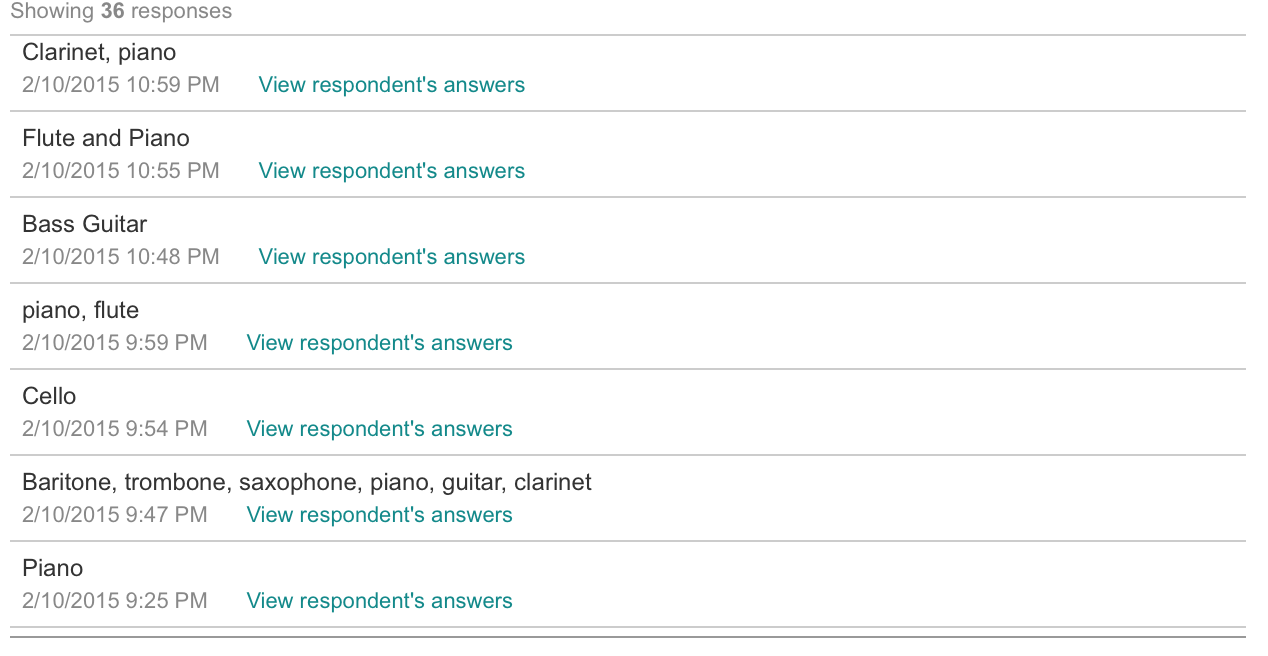
\includegraphics[width=\textwidth]{survey_results/instruments}
\caption{Summary of Instruments each person played}	
\label{fig:instruments}
\end{figure}
The first question, shown in figure \ref{fig:instruments}, asked the person what instruments he or she plays. The list contains a wide range, which is important as only asking a few instrumentalists would yield very different results.

The next question, shown in figure \ref{fig:range}, asked the person what range and key their instruments have. Range is an indication of the number of octaves the instrument is able to produce. This information is useful to know in order to analyse differences, for example instruments which are not of the same family but have a similar range might have similarities later in the survey.
\begin{figure}[H]
\centering
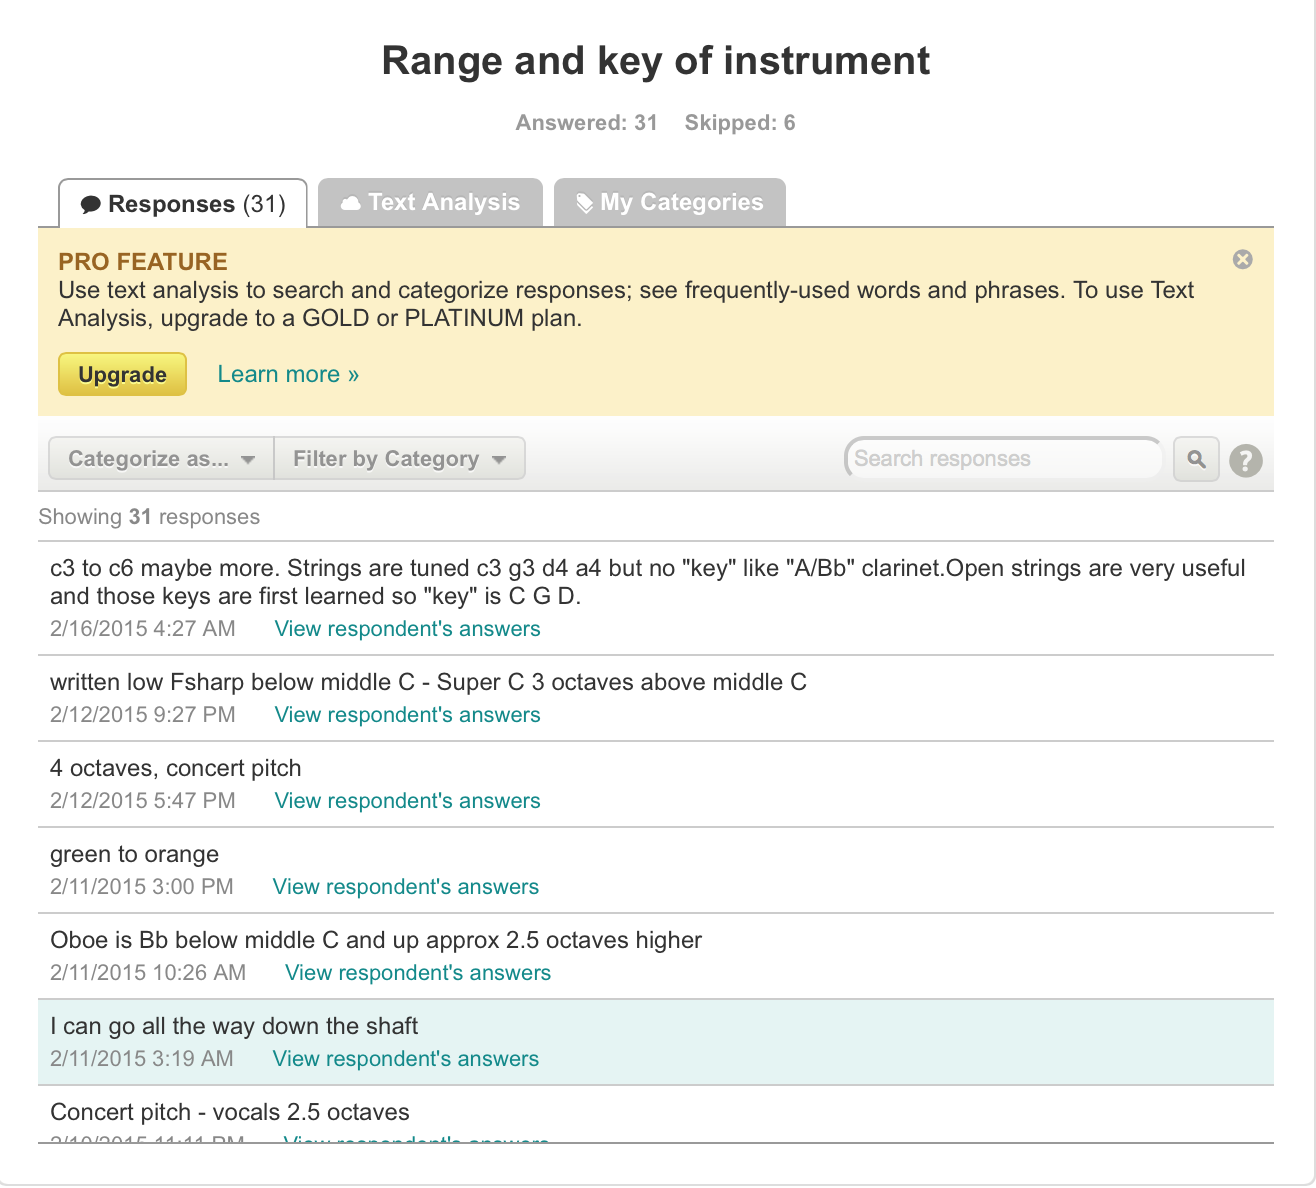
\includegraphics[width=\textwidth]{survey_results/range_key}
\caption{Summary of Range/Key}	
\label{fig:range}
\end{figure}

The third question, answers in figure \ref{fig:grade} asked the person's ability. "Graded" exams indicate Associated Board of the Royal Schools of Music examinations which give an indication of skill, 1 being the lowest and 8 being the highest.

\begin{figure}[H]
\centering
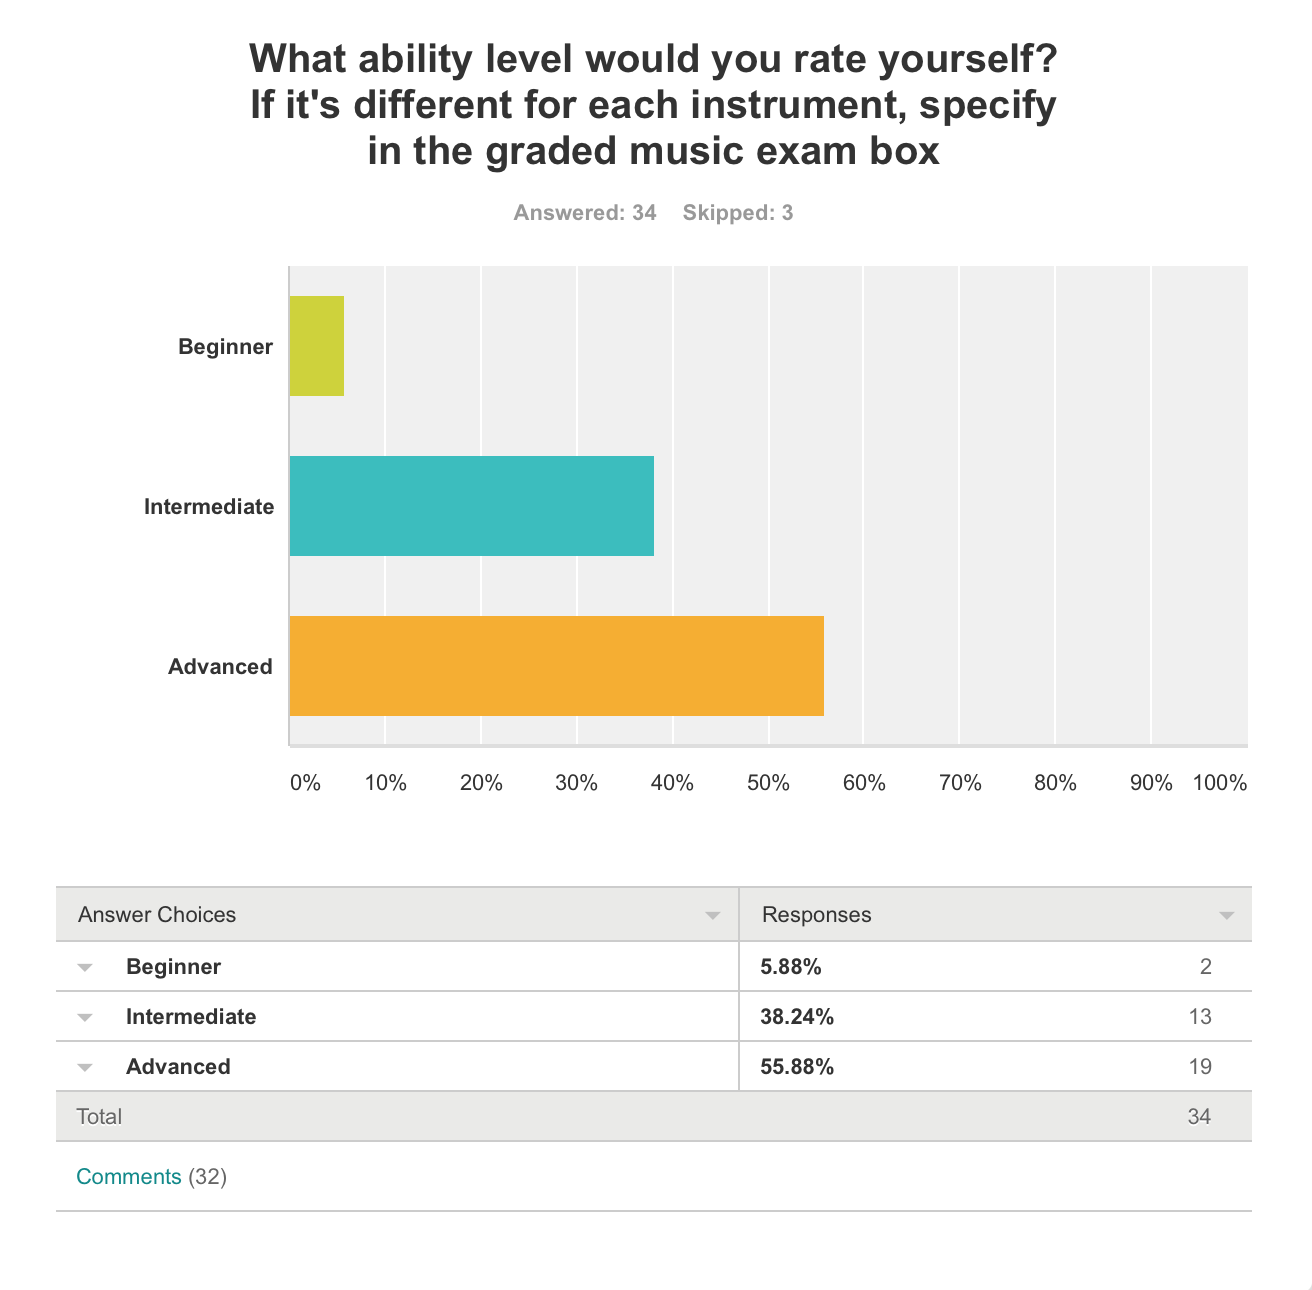
\includegraphics[width=\textwidth]{survey_results/ability}
\caption{Summary of Abilities}	
\label{fig:range}
\end{figure}

After this, the survey contained a series of questions where the user was asked to rate the difficulty - easy, medium or hard. A comments section was provided in order to give more specifics, particularly for instruments which had a particular reason for the difficulty grading.

\begin{figure}[H]
\centering
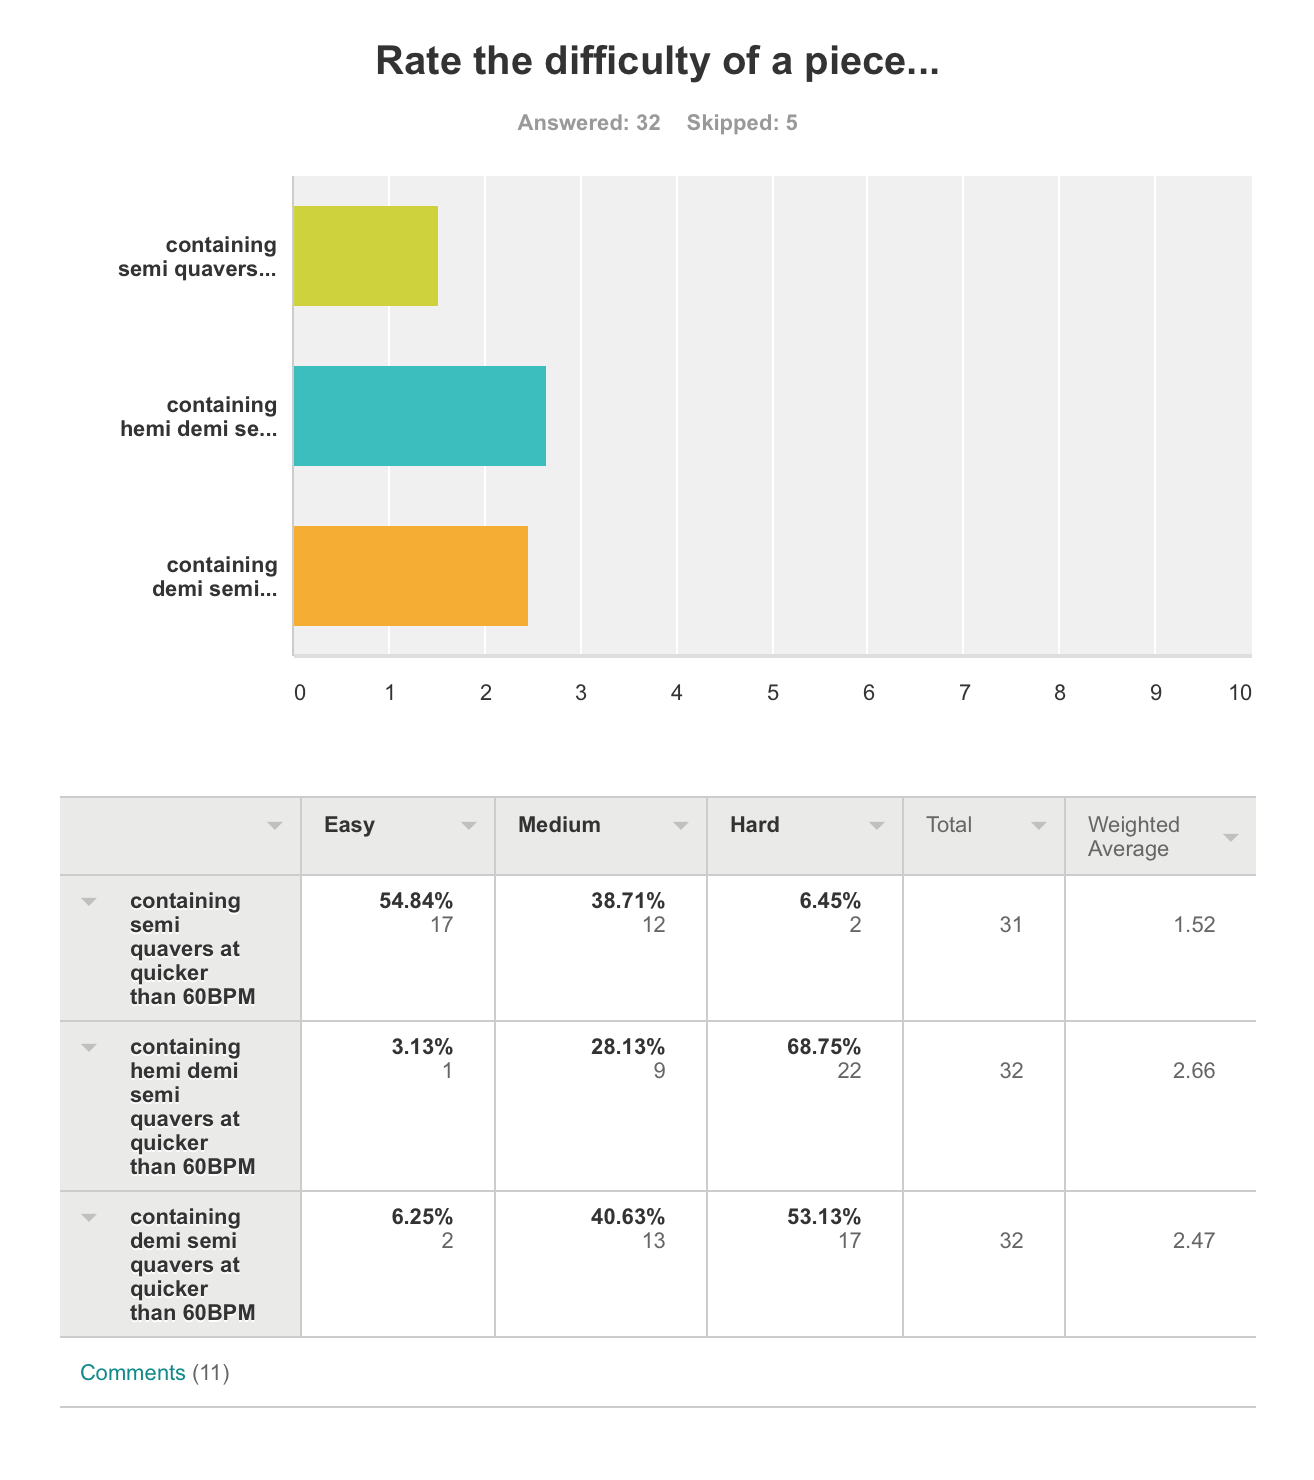
\includegraphics[width=\textwidth]{survey_results/rhythm}
\end{figure}

\begin{figure}[H]
\centering
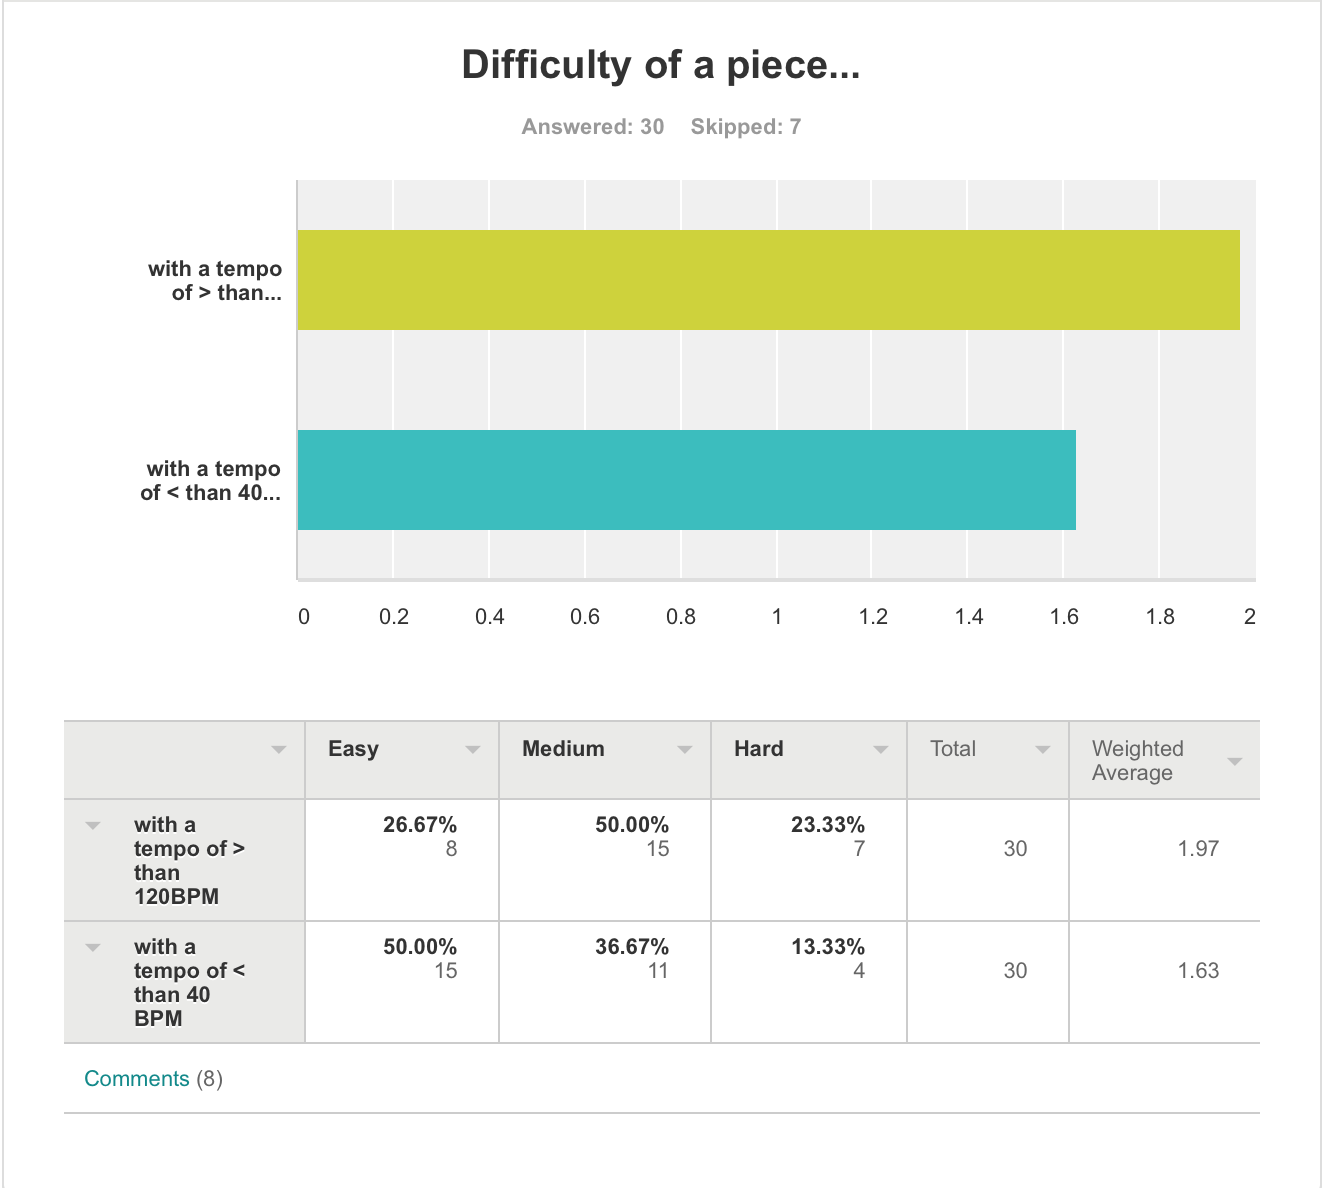
\includegraphics[width=\textwidth]{survey_results/tempo}
\end{figure}

\begin{figure}[H]
\centering
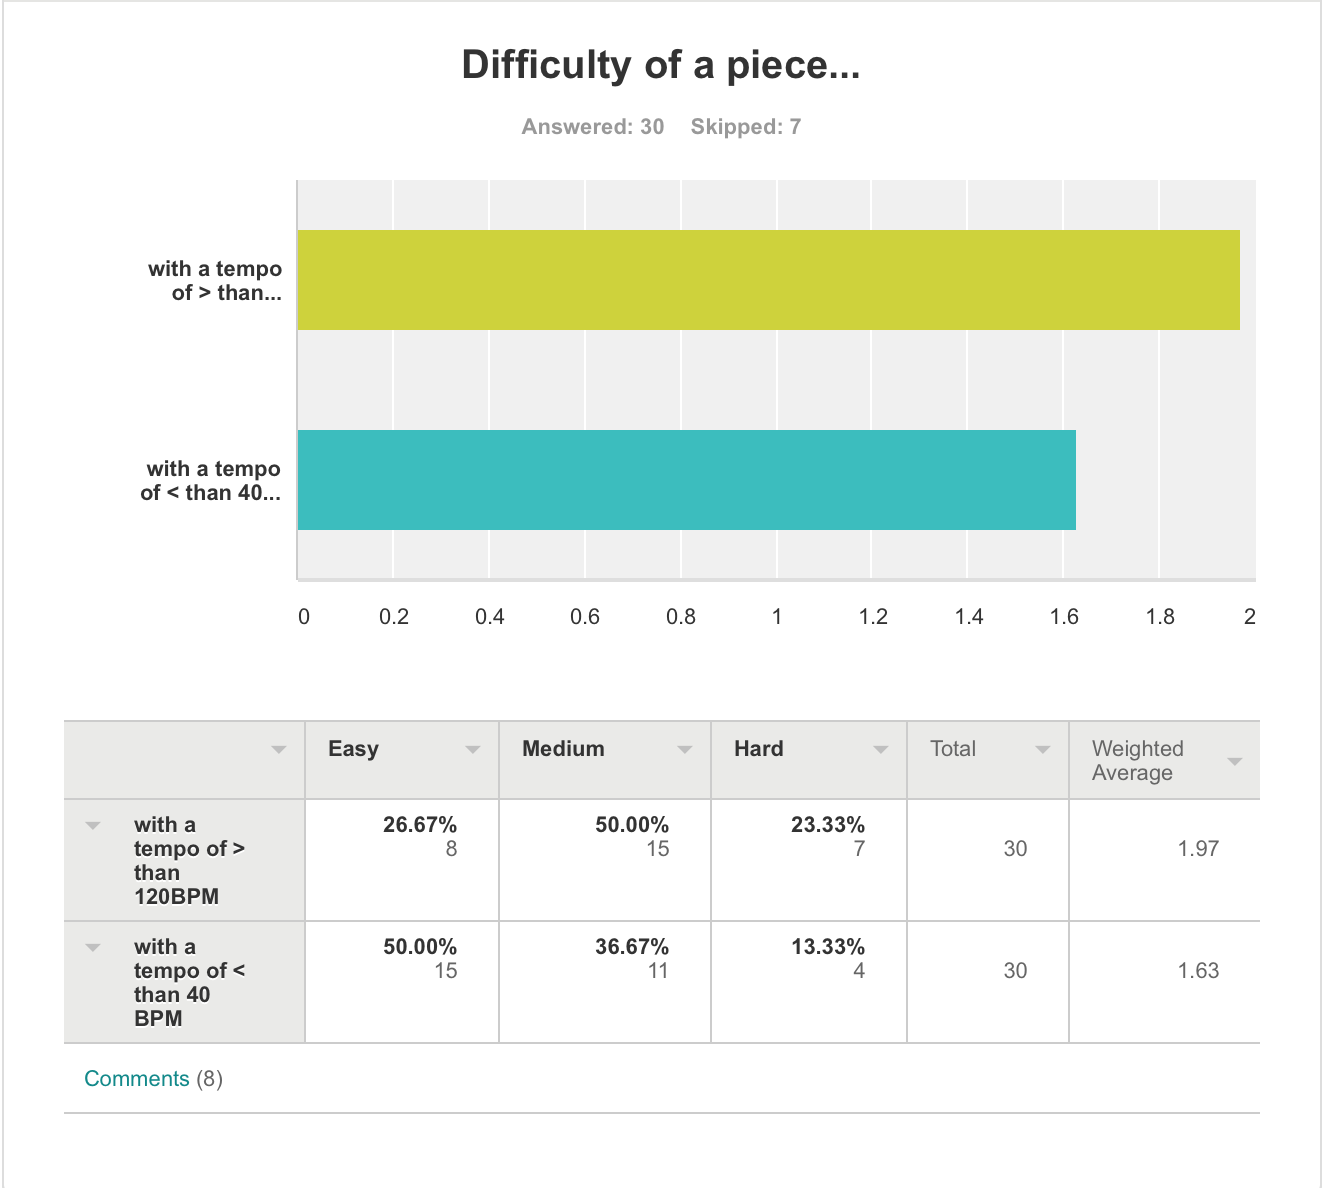
\includegraphics[width=\textwidth]{survey_results/tempo}
\end{figure}

\begin{figure}[H]
\centering
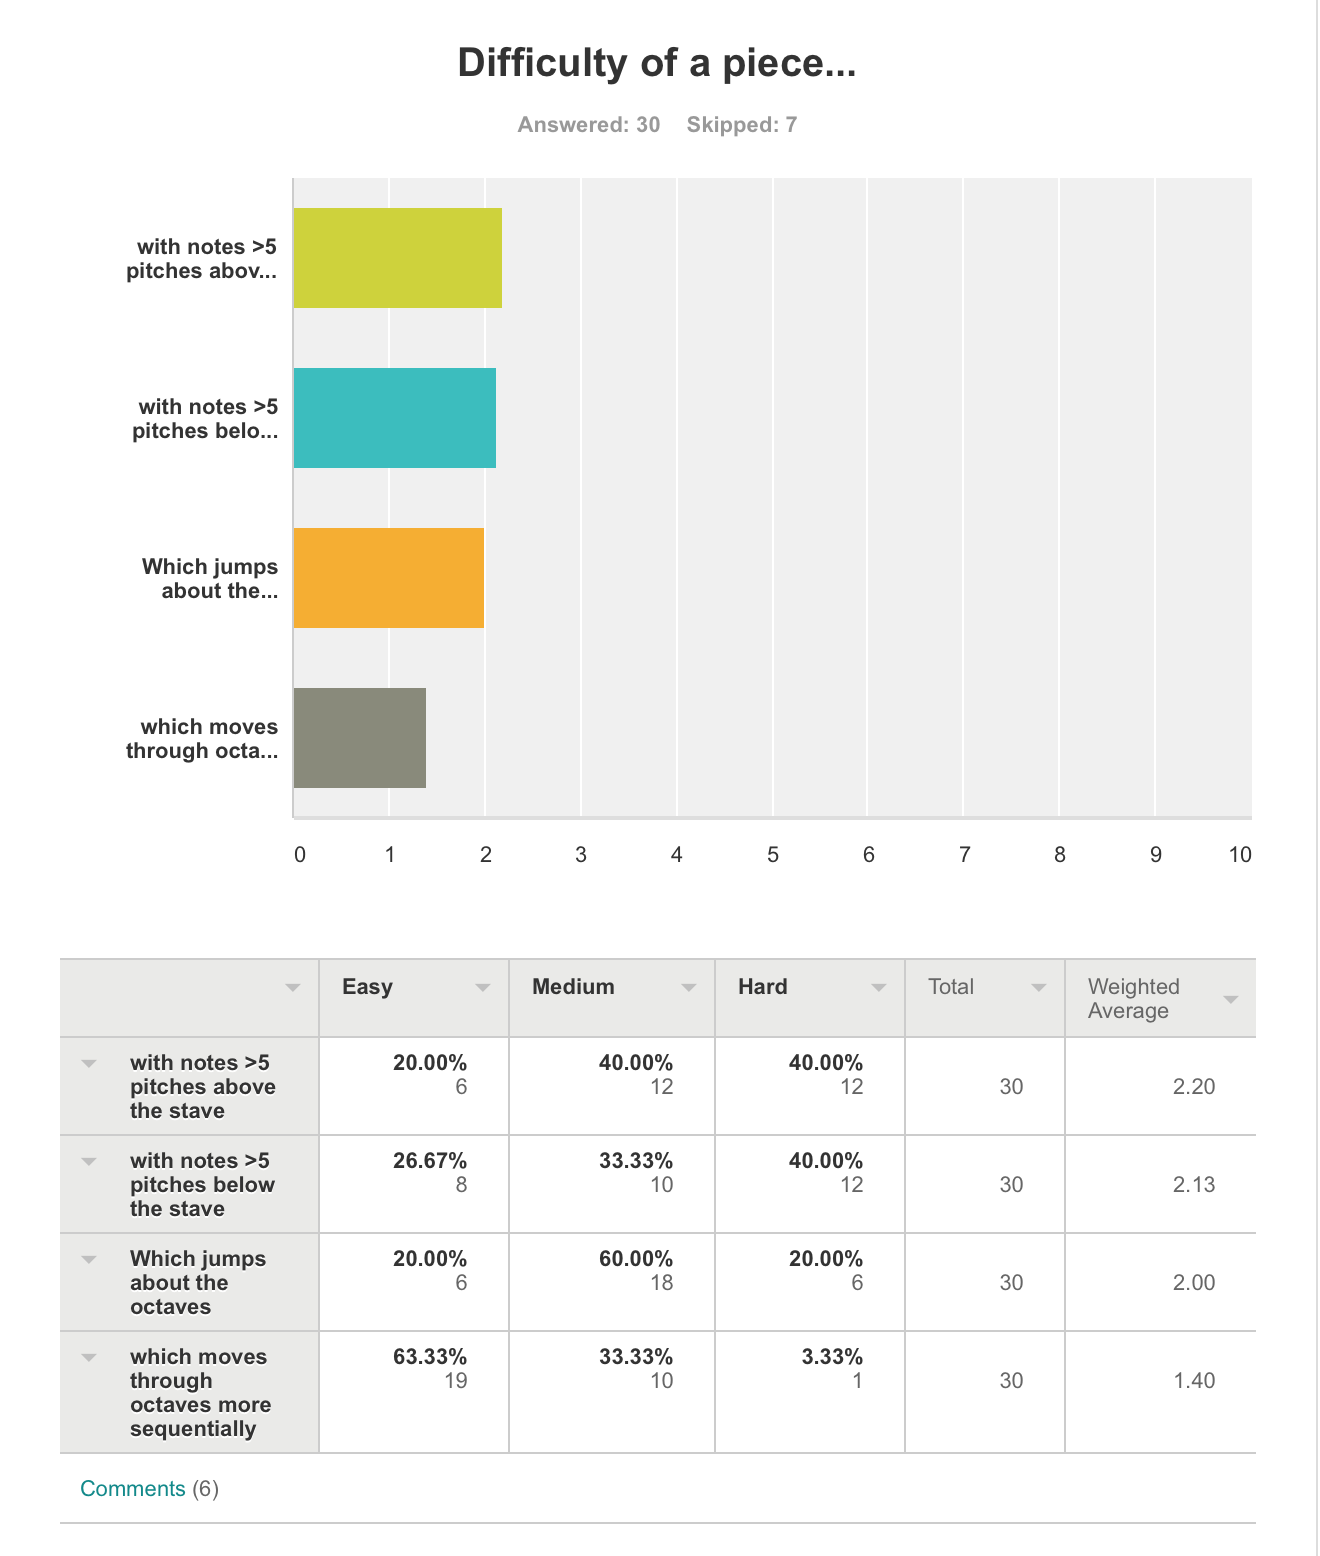
\includegraphics[width=\textwidth]{survey_results/pitches}

\end{figure}

\begin{figure}[H]
\centering
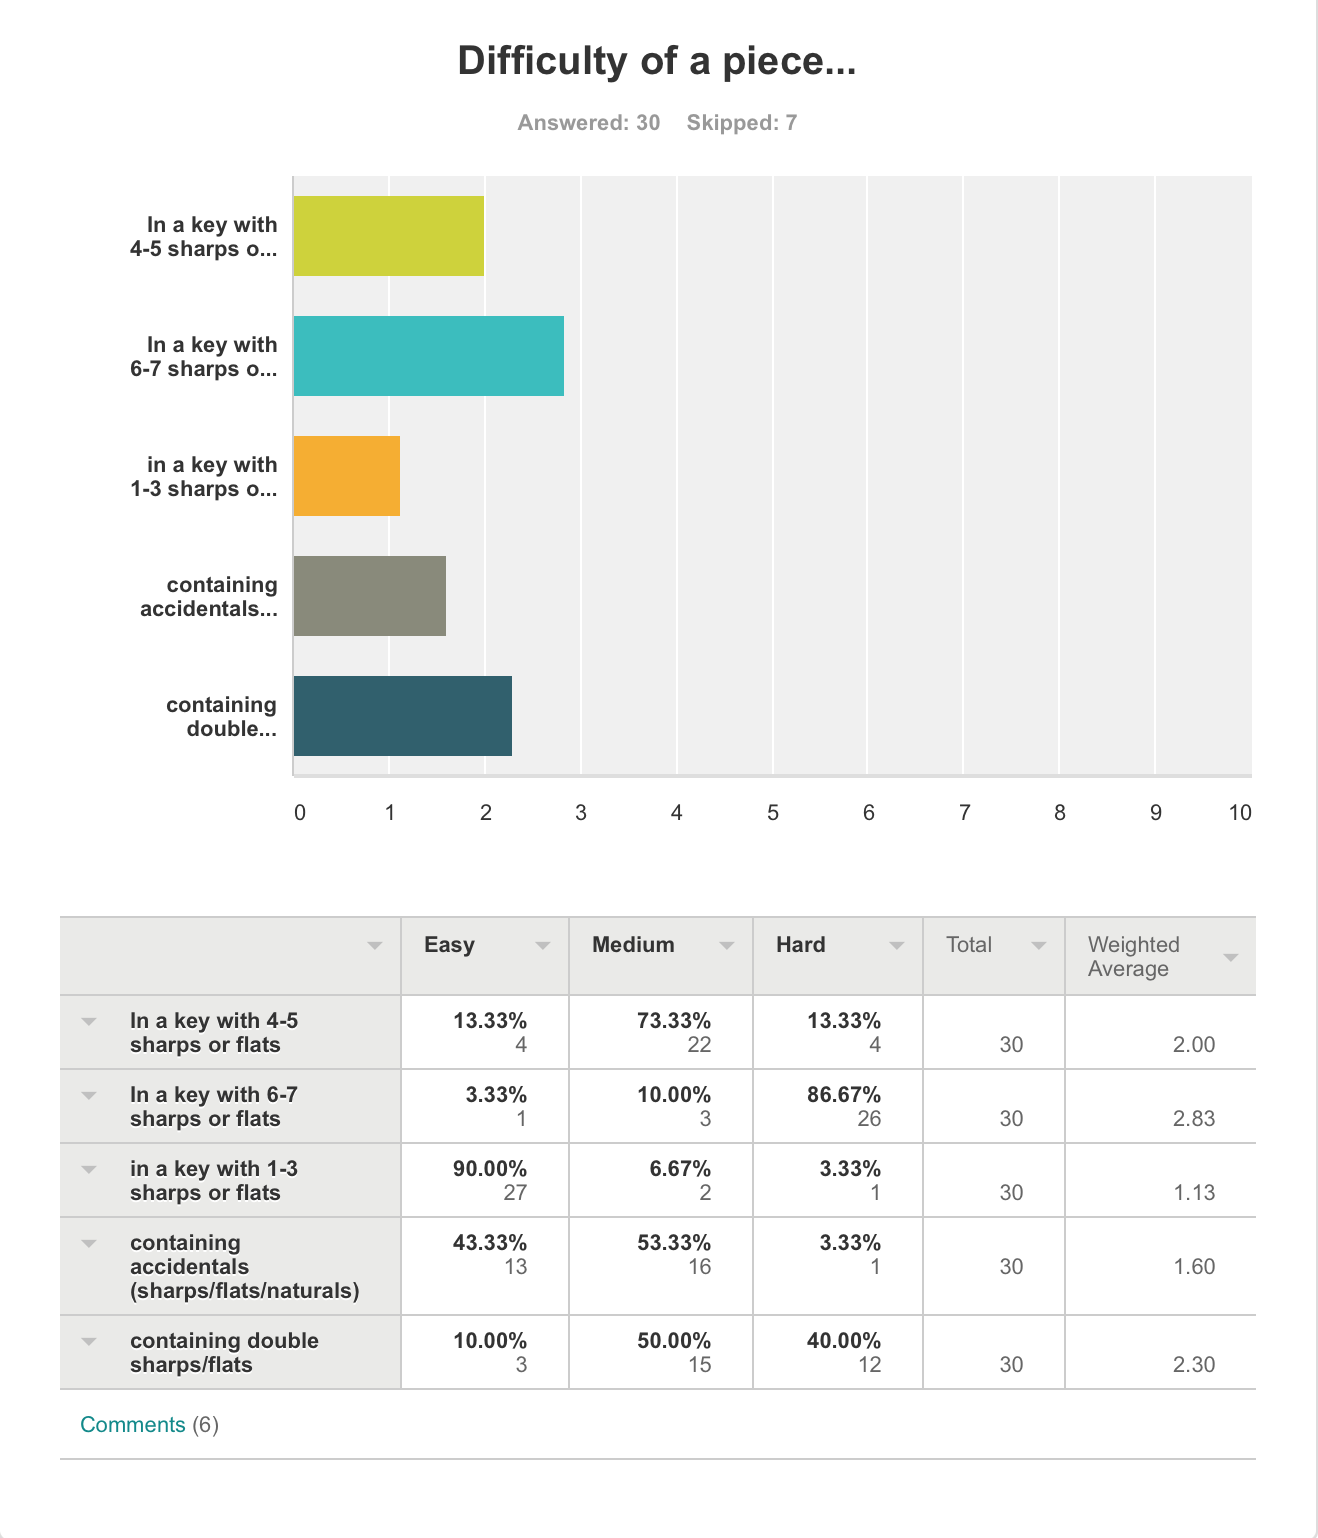
\includegraphics[width=\textwidth]{survey_results/keysig}
\end{figure}

The final question provided a space for the participant to enter any details of their instrument which were not answered by any of the other questions. 
\begin{figure}[H]
\centering
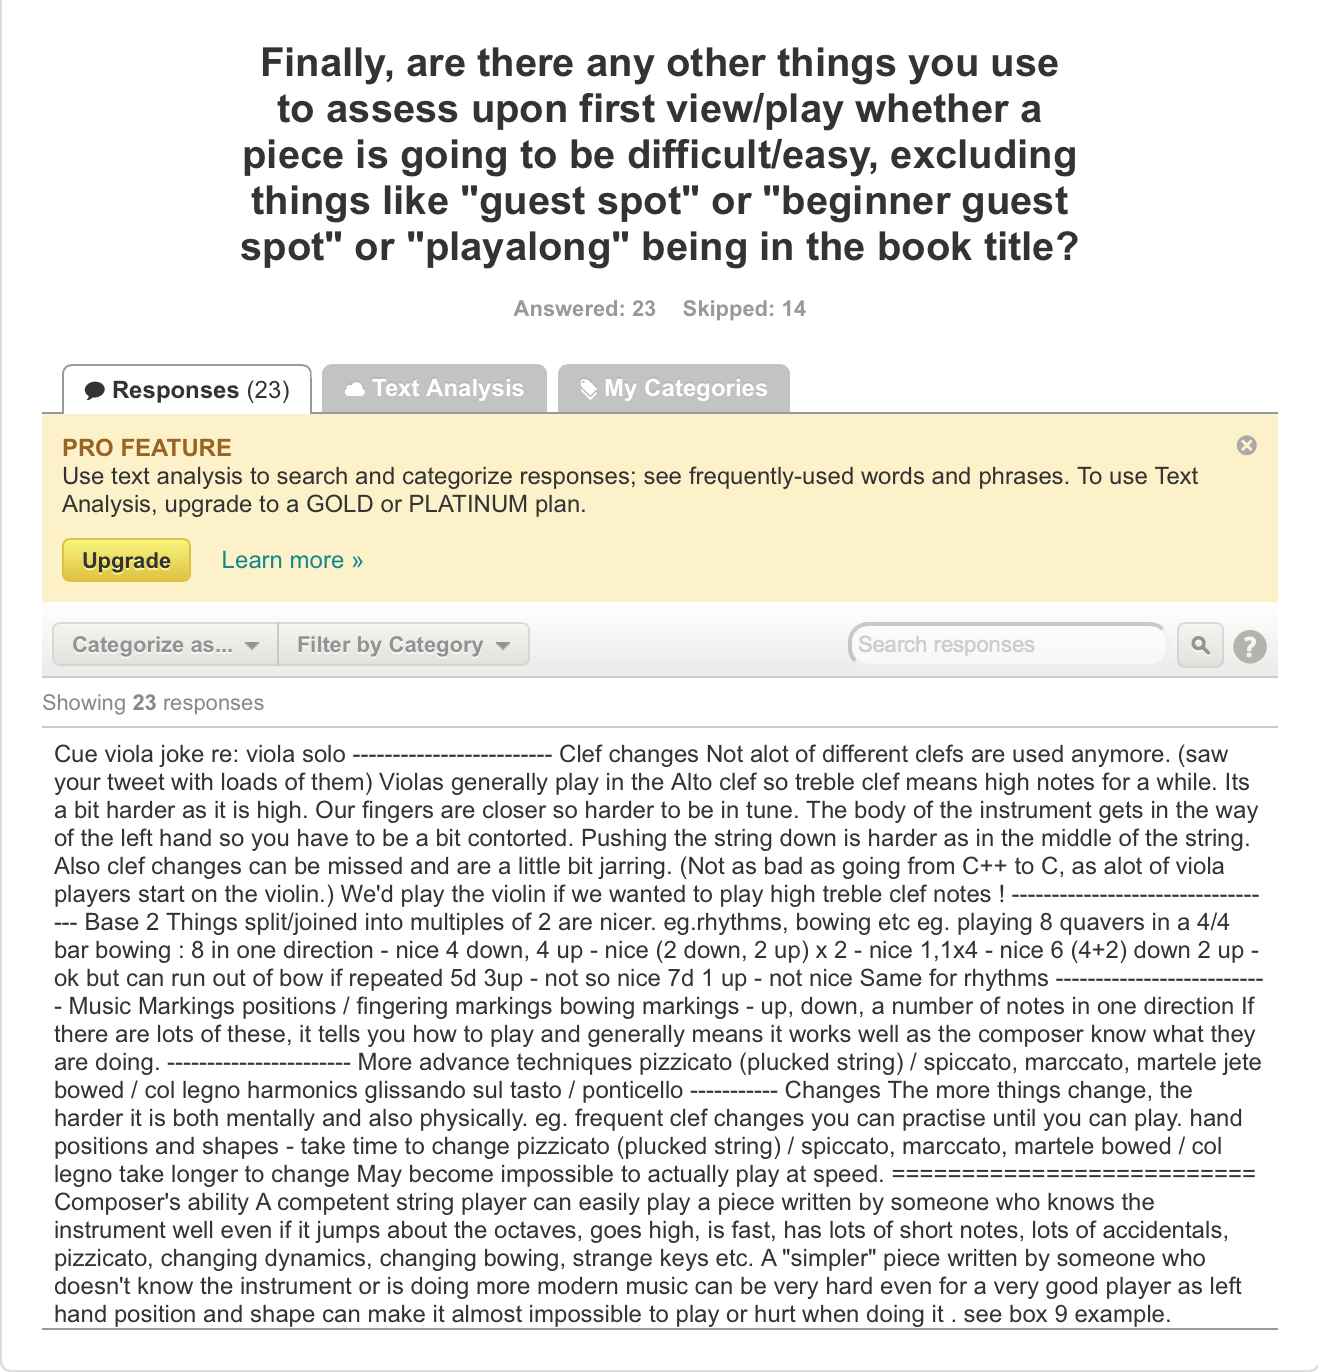
\includegraphics[width=\textwidth]{survey_results/final_q}
\end{figure}
\floatstyle{plain}
\restylefloat{figure}
\section{User guide}
\includepdf[pages=-]{user_guide/userguide.pdf}
\section{Test cases}
Table \ref{table:testcases} gives a brief explanation of all the current testcases being used to validate the system against real world applications. Listing \ref{code:keysig} gives one example, keySignatures.xml, of a musicXML file.
\begin{table}[H]
\centering
\begin{tabu}to 1.0\textwidth{| X[l] | X[l] |} \hline
{Name} & {Purpose} \\ \hline	
Accidentals.xml & Tests system properly handles all possible accidentals attached to notes \\ \hline
GraceNotes.xml & Tests gracenotes attached to notes \\ \hline
Tremolo.xml & tests tremolo on notes \\ \hline
TrillsFermataOrnaments.xml & tests trills, fermatas (pauses) and other ornaments on notes \\ \hline
arpeggiosAndGlissandos.xml & tests arpeggios and glissandos on notes \\ \hline
barlines.xml & tests different barlines applied to measures \\ \hline
beams.xml & tests beaming of notes (quavers, semi quavers etc) \\ \hline
breathMarks.xml & tests breathmark notation next to notes \\ \hline
clefs.xml & tests all possible clef types \\ \hline
duration\_and\_stem\_direction.xml & tests duration of notes and their stem (stick) direction) \\ \hline
dynamics.xml & tests dynamics (loud and quiet) and their position in a measure \\ \hline
fingering.xml & fingering notation specific to string instruments \\ \hline
keySignatures.xml & tests all key signatures and their names are correct \\ \hline
lines.xml & tests a variety of lines over bars, such as pedal marks and repeat alternative bars \\ \hline
multiple\_parts.xml & tests how the system handles more than one instrumental part \\ \hline
noteheads.xml & tests all possible changes to the shape of the notehead \\ \hline
repeatMarks.xml & tests repeat marks are loaded correctly (i.e, points at which the player must go back to a specific sign and play it again) \\ \hline
text.xml & tests text markings, such as dynamic and tempo markings like "andante", but also things like lyrics \\ \hline
tuplets.xml & tests tuplets, where a note must be played differently to how it is notated according to its tuplet value \\ \hline
two\_staves\_one\_part.xml & tests loading of two staves in one part, such as pianos and harpsichords \\ \hline
\end{tabu}
\caption{All testcases currently in use}	
\label{table:testcases}
\end{table}

\lstset{
    language=xml,
    tabsize=3,
    %frame=lines,
    caption=key signature testcase,
    label=code:keysig,
    frame=shadowbox,
    rulesepcolor=\color{gray},
    xleftmargin=20pt,
    framexleftmargin=15pt,
    keywordstyle=\color{blue}\bf,
    commentstyle=\color{OliveGreen},
    stringstyle=\color{red},
    numbers=left,
    numberstyle=\tiny,
    numbersep=5pt,
    breaklines=true,
    showstringspaces=false,
    basicstyle=\footnotesize,
    emph={food,name,price},emphstyle={\color{magenta}}}
    \lstinputlisting{testcases/keySignatures.xml}
\end{appendices}